% -*- coding: utf-8; -*-

\chapter{Compressão de Provas e Dados}
\label{cap:comp_prov_dado}

\section{Compressão Horizontal}
\label{sec:comp_hor}

Proposta por Gordeev e Haeusler \cite{GordeevH16}, a \textit{Compressão Horizontal}\footnote{Além da referência \cite{GordeevH16}, a descrição da Compressão Horizontal apresentada neste trabalho é originada de notas não publicadas \cite{GorHaeHCNonPub} e comunicação pessoal com Haeusler} (CH) é uma técnica de compressão de provas em dedução natural da M$\supset$ que utiliza grafos direcionados para representar as provas. Essa técnica de compressão é utilizada como uma ferramenta para provar a conjectura $NP = PSPACE$. Dada a prova de uma tautologia qualquer da M$\supset$, que pode possuir tamanho exponencial em relação ao tamanho da conclusão, o objetivo da CH é que a prova resultante da compressão possua tamanho polinomialmente limitado em relação ao tamanho da conclusão. Na representação de provas utilizando grafos direcionados, cada vértice do grafo é rotulado com uma fórmula. O processo de compressão ocorre através da fusão de vértices rotulados com fórmulas idênticas que estejam localizados na mesma seção horizontal da derivação, iniciando no nível da conclusão e indo até os níveis das hipóteses.

\subsection{Definições sobre grafos}

Esta seção apresenta os principais conceitos sobre grafos utilizados para apresentar a Compressão Horizontal.

\begin{definition}{\textbf{Grafo.}}
Um \textit{grafo} é uma tripla ordenada $G = \langle V(G), A(G), I_G\rangle$, onde $V(G)$ é um conjunto não vazio, $V(G)$ e $A(G)$ são conjuntos disjuntos e $I_G$ é uma função de incidência que associa cada elemento de $A(G)$ a um par não ordenado de elementos de $V(G)$, $I_G: A(G) \rightarrow V(G) \times V(G)$. Elementos de $V(G)$ são chamados de \textit{vértices} e os elementos de $A(G)$ são chamados de \textit{arestas}.
\end{definition}

\begin{example}
Se $V(G) = \{v_1, v_2, v_3\}$, $A(G) = \{a_1, a_2, a_3\}$ e $I_G$ é dado por $I_G(a_1) = (v_1, v_2)$, $I_G(a_2) = (v_2, v_3)$ e $I_G(a_3) = (v_1, v_2)$, então $\langle V(G), A(G), I_G\rangle$ é um grafo.
\end{example}

Essa definição de grafo permite que existam mais de uma aresta entre um mesmo par de vértices (multiarestas), além disso, permite que existam arestas que conectam um vértice a ele mesmo (laços). Grafos que que possuem multiarestas e/ou laços são chamados de \textit{multigrafos}. Grafos que permitem no máximo uma aresta entre cada par de vértices são chamados de grafos simples.

\begin{definition}{\textbf{Grafo simples.}}
Um \textit{grafo simples} é um par ordenado $\langle V(G), A(G)\rangle$, onde $A(G)$ é um subconjunto de pares não ordenados de $V(G)$, $A(G) \subseteq V(G) \times V(G)$. Se $a, b \in V(G)$ e $(a, b) \in A(G)$, então $a \neq b$.
\end{definition}

Os grafos que possuem o conjunto de arestas composto por pares não ordenados do conjunto de vértices são chamados de \textit{grafos não direcionados}. Os grafos com o conjunto de arestas composto por pares ordenados são chamados de \textit{grafos direcionados}.

\begin{definition}{\textbf{Grafo direcionado.}}
Um \textit{grafo direcionado} é um par ordenado $\langle V(G), A(G)\rangle$, onde $A(G)$ é um subconjunto de pares ordenados de $V(G)$, $A(G) \subseteq V(G) \times V(G)$. Se $a, b \in V(G)$ e $(a, b) \in A(G)$, então $(a, b) \neq (b, a)$.
\end{definition}

\begin{example}
\label{ex:grafo_ds}
Se $V(G) = \{v_1, v_2, v_3\}$, $A(G) = \{(v_1, v_3), (v_2, v_3), (v_2, v_1)\}$, onde cada elemento de $A(G)$ é um par ordenado, então $\langle V(G), A(G)\rangle$ é um grafo simples e um grafo direcionado.
\end{example}

Nas definições seguintes, os grafos são direcionados e simples. 

\begin{definition}{\textbf{Grafos rotulados.}}
Dado um grafo $(V(G), A(G))$ e um conjunto de rótulos $R$. $\langle V(G), A(G), r_v\rangle$ é um grafo rotulado nos vértices, onde $r_v$ é uma função que associa cada vértice a um rótulo de $R$, $r_v: V(G) \rightarrow R$. Um grafo rotulado nas arestas possui uma função $r_a$ das arestas para os rótulos, $r_a: A(G) \rightarrow R$.
\end{definition}

\begin{definition}{\textbf{Grafos coloridos.}}
Seja um grafo $G = \langle V(G), A(G)\rangle$, um grafo com arestas coloridas possui uma coloração de arestas $c$, $c: A(G) \rightarrow S$, onde $S$ é um conjunto de cores. Um grafo $G$ é um grafo com arestas $n$-coloridas, se $|S| = n$.
\end{definition}

A definição anterior de grafos coloridos nas arestas é um pouco diferente da usual, pois permite que arestas da mesma cor sejam adjacentes. Em um grafo direcionado, duas arestas são adjacentes se possuem um vértice em comum.

\begin{definition}{\textbf{Caminho.}}
Dado um grafo $\langle V(G), A(G)\rangle$. Um \textit{caminho} com tamanho $n$ é uma lista de $n$ arestas de $A(G)$, $\langle (v^1_1, v^1_2), ..., (v^n_1, v^n_2)\rangle$, onde para todo $i$, $j$ de 1 até $n$, $v^i_2 = v^{i+1}_1$, $v^i_1 \neq v^j_1$ e $(v^i_1, v^i_2) \neq (v^j_1, v^j_2)$.
\end{definition}

\begin{definition}{\textbf{Árvore.}}
Dado um grafo $\langle V(G), A(G))$, $(V(G), A(G), r\rangle$ é uma \textit{árvore}, onde $r \in V(G)$ e para todo $v \in V(G)$, existe apenas um caminho de $r$ para $v$. 
\end{definition}

\begin{definition}{\textbf{Grau de saída.}}
Dado um grafo direcionado $\langle V(G), A(G)\rangle$. O \textit{grau de saída} de um vértice $v \in V$ é a quantidade de arestas que possuem $v$ na primeira posição do par ordenado.
\end{definition}

\begin{example}
Considere o grafo ordenado do Exemplo \ref{ex:grafo_ds}. Os vértices $v_1$, $v_2$ e $v_3$ possuem o grau de saída igual a, respectivamente, $1$, $2$ e $0$.
\end{example}

\begin{definition}{\textbf{Grau de entrada.}}
Dado um grafo direcionado $\langle V(G), A(G)\rangle$. O \textit{grau de entrada} de um vértice $v \in V$ é a quantidade de arestas que possuem $v$ na segunda do par ordenado.
\end{definition}

\begin{example}
Considere o grafo ordenado do Exemplo \ref{ex:grafo_ds}. Os vértices $v_1$, $v_2$ e $v_3$ possuem o grau de entrada igual a, respectivamente, $1$, $0$ e $2$.
\end{example}

No restante do texto, para um grafo $G$, omitimos a identificação de $G$ nos conjuntos de vértices e arestas. Um grafo $G$ é denotado por $G = (V, A)$. 

\subsection{Grafos direcionados como derivações}

No estilo de Gentzen-Prawitz, uma derivação é uma árvore onde os nós e as arestas são rotulados com, respectivamente, fórmulas e regras de inferência. Baseado nesse estilo, uma derivação na CH é representada por um grafo direcionado com arestas coloridas que possui fórmulas como  rótulos nos vértices.

Nas definições a seguir, considere as seguintes funções que mapeiam fórmulas e conjunto de fórmulas em suas respectivas subfórmulas. $Sub_f$ é uma função que mapeia uma fórmula em um conjunto com todas as suas subfórmulas; $Sub_c$ é uma função que mapeia um conjunto de fórmulas em um conjunto da união dos conjuntos de subfórmulas de cada fórmula.

\begin{example}
Seja a fórmula $\alpha = A \supset (B \supset C)$. O conjunto de subfórmulas de $\alpha$ é definido por: $$Sub_f(\alpha) = \{A,\; B,\; C,\; B\supset C,\; A \supset (B \supset C)\}$$
\end{example}

\begin{example}
Seja o conjunto de fórmulas $$\Delta = \{(A \supset (B \supset C)),\; (B \supset (A \supset C))\}$$ O conjunto da união dos conjuntos de subfórmulas de cada fórmula de $\Delta$ é definido por: $$Sub_c(\Delta) = \{A,\; B,\; C,\; B\supset C,\; A \supset (B \supset C),\; A \supset C,\; B \supset (A \supset C)\}$$
\end{example}

Sejam um grafo direcionado $\langle V, A\rangle$ e um subconjunto das arestas $A' \supseteq A$. As funções $gs: V \times A' \rightarrow \mathbb{N}$ e $ge: V \times A' \rightarrow \mathbb{N}$ mapeiam um vértice em seus graus, respectivamente, de saída e entrada, considerando apenas as arestas em $V'$.

\begin{definition}{\textbf{Grafo de derivação.}}
Seja uma derivação $\Pi$ de $\Gamma \vdash \alpha$, um \textit{grafo de derivação} é um grafo simples, direcionado, colorido nas arestas e rotulado nos vértices $\langle V, A, r, c, l\rangle$, onde: $V$ é o conjunto não vazio de vértices; $A$ é o conjunto de arestas, $A \subseteq V \times V$; $c$ é a função de coloração das arestas, $c: A \rightarrow \{0, 1\}$, onde as arestas do conjunto $A_D = \{\langle u, v\rangle \;|\; c(\langle u, v\rangle) = 0\}$ são chamadas de \textit{arestas de dedução} e as arestas do conjunto $A_d =  \{\langle u, v\rangle \;|\; c(\langle u, v\rangle) = 1\}$ são chamadas de \textit{arestas de descarte}; o conjunto de arestas é formado pela união dos conjuntos das arestas de dedução e de descarte, $A = A_D \cup A_d$; toda aresta é exclusivamente de dedução ou exclusivamente de descarte, $A_D \cap A_d = \emptyset$; $\langle V, A_D, r \rangle$ é uma árvore; $l$ é a função que rotula os vértices com as fórmulas, $l:V \rightarrow Sub_{c}(\Gamma) \cup Sub_{f}(\alpha)$; tal que:

\begin{enumerate}
    \item O vértice $r$ não possui arestas dedutivas saindo dele, $gs(A_D, r) = 0$, e possui a conclusão da derivação como rótulo, $l(r) = \alpha$.
    \item Todo vértice $v \in V$ possui $ge(A_D, v)$ igual a 0, 1 ou 2.
    % \item $\forall v \in V(.ge_D(v) = 0 \lor ge_D(v) = 1 \lor ge_D(v) = 2)$.
    \item Para todo vértice $v \in V$, se $ge(A_D, v) = 1$, então $ge(A_d, v) \geq 1$ e $l(v)$ é a conclusão de uma regra $\mysupset{-I}$, tal que
    
    \begin{center}
        \begin{tikzpicture}[-triangle 60, node distance=2.2cm and 1cm, auto]
            % \tikzstyle{every state}=[circle,thick,minimum size=5mm, text=black,minimum width=1cm]
            \node[state, inner sep=1mm,minimum size=1.2cm, label=right:$x_1$] (A) {$\alpha$};
            \node[state, draw=none,fill=none] (D) [right of=A] {...};
            \node[state, inner sep=1mm,minimum size=1.2cm, dotted, label=right:$x_n$] (E) [right of=D] {$\alpha$};
            \node[state, inner sep=1mm,minimum size=1.2cm, label=right:$w$] (B) [below of=D] {$\beta$};
            \node[state, inner sep=1mm,minimum size=1.2cm, label=right:$v$] (C) [below of=B] {$\alpha \supset \beta$};
            
            \path[-latex]  (A) edge [bend right=30, thick, left]  node {{$a1_d$}} (C);
            \path[-latex]  (B) edge [thick] node {$a_D$} (C);
            \path[-latex]  (E) edge [bend left=30, loosely dotted, thick]  node {{$an_d$}} (C);
            \path[-latex]  (A) edge [bend left=20, dashed, thick] node {} (B);
            \path[-latex]  (E) edge [bend right=20, loosely dotted, thick] node {} (B);
        \end{tikzpicture}
    \end{center}
    
    o rótulo do vértice $w$ associado a $v$ por uma aresta de dedução ($a_D$) é idêntico ao consequente de $l(v)$; os rótulos dos vértices ($x_1, ..., x_n$) associados a $v$ por arestas de descarte ($a1_d, ..., an_d$) são idênticos ao antecedente de $l(v)$.
    
    \item Para todo vértice $v \in V$, se $ge(A_D, v) = 2$, então $l(v)$ é a conclusão de uma regra $\mysupset{-E}$, tal que
    
    \begin{center}
        \begin{tikzpicture}[-triangle 60, node distance=3cm and 1cm, auto]
            % \tikzstyle{every state}=[circle,thick,minimum size=5mm, text=black,minimum width=1cm]
            \node[state, inner sep=1mm,minimum size=1.2cm, label=right:$v$] (A) {$\beta$};
            \node[state, inner sep=1mm,minimum size=1.2cm, label=right:$w_1$] (B) [above left of=A] {$\alpha$};
            \node[state, inner sep=1mm,minimum size=1.2cm, label=right:$w_2$] (C) [above right of=A] {$\alpha \supset \beta$};
            
            \path[-latex]  (B) edge [thick, left]  node {{$a1_D$}} (A);
            \path[-latex]  (C) edge [thick]  node {{$a2_D$}} (A);
        \end{tikzpicture}
    \end{center}
    
    sejam os vértices $w_1$ e $w_2$ associados a $v$, onde $|l(w_1)| < |l(w_2)|$, o rótulo de $w_1$ é idêntico ao antecedente de $l(w_2)$, o rótulo de $v$ é idêntico ao consequente de $l(w_2)$.
    
    \item Para todo vértice $v \in V$, se $ge(A_D, v) = 0$ e $gs(A_d, v) = 0$, então $l(v)$ é uma hipótese de $\Pi$.
\end{enumerate}
\end{definition}

Para exemplificar a representação de derivações por Grafos de Prova, a Figura \ref{fig:exe_gra_pro} mostra o grafo que representa a derivação de $$\vdash (A \supset (B \supset C)) \supset (B \supset (A \supset C))$$ As arestas com linhas tracejadas são arestas de descarte.

\begin{figure}[ht]
    \begin{center}
        \begin{tikzpicture}[auto, elliptic state/.style={draw,ellipse}]
            % \tikzstyle{every state}=[circle,thick,minimum size=5mm, text=black,minimum width=1cm]
            \node[elliptic state] (ABCBAC) {$(A\supset(B\supset C)) \supset (B \supset (A\supset C))$};
            \node[elliptic state] (BAC) [above = 1cm of ABCBAC] {$B \supset (A\supset C)$};
            \node[elliptic state] (AC) [above = 1cm of BAC] {$A\supset C$};
            \node[elliptic state] (C) [above = 1cm of AC] {$C$};
            \node[elliptic state] (C) [above = 1cm of AC] {$C$};
            \node[elliptic state] (B) [above left = 1cm of C] {$B$};
            \node[elliptic state] (BC) [above right = 1cm of C] {$B\supset C$};
            \node[elliptic state] (ABC) [above right = 1cm of BC] {$A\supset(B\supset C)$};
            \node[elliptic state] (A) [above left = 1cm of BC] {$A$};
            
            % \node[state, inner sep=1mm,minimum size=1.2cm, label=right:$w_2$] (C) [above right of=A] {$\alpha \supset \beta$};
            
            \path[-latex]  (ABC) edge [thick] (BC);
            \path[-latex]  (A) edge [thick] (BC);
            \path[-latex]  (BC) edge [thick] (C);
            \path[-latex]  (B) edge [thick] (C);
            \path[-latex]  (C) edge [thick] (AC);
            \path[-latex]  (AC) edge [thick] (BAC);
            \path[-latex]  (BAC) edge [thick] (ABCBAC);
            
            \path[-latex]  (B) edge [dashed, bend right=30] (BAC);
            \path[-latex]  (A) edge [dashed, bend right=100] (AC);
            \path[-latex]  (ABC) edge [dashed, bend left=30] (ABCBAC);
        \end{tikzpicture}
    \end{center}
    \caption{Exemplo de grafo de derivação}
    \label{fig:exe_gra_pro}
\end{figure}

Seja uma derivação $\Pi$ de $\Gamma \vdash \alpha$, a conclusão $\alpha$ depende do conjunto de hipóteses $\Gamma$. Em um grafo de derivação que representa $\Pi$, o conjunto de hipóteses é composto pelos rótulos dos vértices que não possuem arestas de dedução incidentes e que não foram descartados por arestas de descarte. No entanto, as arestas de descarte ($A_d$) adicionam ciclos no grafo $\langle V, A_D \rangle$ (desconsiderando a direção das arestas). 

\begin{definition}
Seja uma derivação $\Pi$ de $\beta$ tendo o conjunto $\Gamma$ de hipóteses. Uma aplicação de $\mysupset{-I}$ é gulosa, se e somente se, produz $\alpha \supset \beta$ e descarta cada ocorrência não descartada de $\alpha$ em $\Pi$ na qual $\beta$ depende.
\end{definition}

\begin{lemma}
Seja uma derivação $\Pi$ de $\alpha$. A derivação $\Pi'$ resultante da transformação de todas as regras $\mysupset{-I}$ de $\Pi$ em gulosas ainda é uma derivação válida de $\alpha$ em M$\supset$ \cite{GorHaeHCNonPub}.
\end{lemma}

Com as regras $\mysupset{-I}$ gulosas, as informações de dependências podem ser diretamente determinadas nos vértices ($V$) ou nas arestas de dedução ($A_D$) e portanto, as arestas de descarte deixam de ser necessárias. As definições a seguir utilizam grafos de provas com todas as regras $\mysupset{-I}$ gulosas.

\vspace{3mm}

\begin{definition}
Seja $\Lambda$ um conjunto de fórmulas de tamanho $n$ e $\mathcal{O}(\Lambda)$ uma ordenação linear das fórmulas de $\Lambda$, $\mathcal{O}(\Lambda) = \{\beta_1, \beta_2, ..., \beta_n\}$. Uma cadeia de \textit{bits} em $\mathcal{O}(\Lambda)$ é uma sequência de \textit{bits} $\langle b_1, b_2, ..., b_n\rangle$, onde cada $b_i \in \{0, 1\}$ com $i$ variando de $1$ até $n$. Para todo conjunto de fórmulas $\Lambda$ de tamanho $n$, existe uma função bijetora $f$ entre o conjunto de todas as cadeias de bits de tamanho \textit{n} e o conjunto das partes de $\Lambda$, $f: B(\mathcal{O}(\Lambda)) \rightarrow \mathcal{P}(\Lambda)$, $f(\langle b_1, ..., b_n\rangle) = \{\beta_i | b_i = 1\}$.
\end{definition}

\begin{example}
Seja $\Lambda = \{A, B, C, (A \supset B)\}$ e uma ordenação linear  $\mathcal{O}(\Lambda) = [(A \supset B), A, C, B]$, onde $(A \supset B)$, $A$, $C$ e $B$ possuem os índices 1, 2, 3 e 4, respectivamente. Para cadeias de \textit{bits} de tamanho 4, a função $f$ da definição anterior possui o seguinte comportamento para as seguintes cadeias de \textit{bits}: $f(\langle 0, 1, 1, 0\rangle) = \{A, C\}$; $f(\langle 1, 0, 1, 0\rangle) = \{(A \supset B), C\}$.
\end{example}

Em uma derivação de $\Gamma \vdash \alpha$, sendo o conjunto $\Lambda = Sub
_{c}(\Gamma) \cup Sub_{f}(\alpha)$, $\mathcal{O}(\Lambda)$ pode ser utilizado para associar cada ocorrência de fórmula com suas respectivas dependências.

Na definição a seguir, considere $b_{\langle \beta \rangle}$ como a cadeia de \textit{bits} que contém apenas o \textit{bit} referente à fórmula $\beta$ igual a 1.

\vspace{3mm}

\begin{definition}{\textbf{Grafo de derivação decorado.}}
Sejam uma derivação $\Pi$ de $\Gamma \vdash \alpha$, um conjunto de fórmulas $\Lambda = Sub_{c}(\Gamma) \cup Sub_{f}(\alpha)$, um grafo de derivação de $\Pi$ $\langle V, A_D, A_d, r, c, l\rangle$ e uma ordenação linear $\mathcal{O}(\Lambda)$. $\langle V, A_D, r, c, l, d \rangle$ é um \textit{grafo de derivação decorado}, onde \textit{d} é uma função que associa cada aresta $(v1, v2) \in A_D$ a uma cadeia de bits que representa as dependências de $l(v1)$, $d: A_D \rightarrow B(\mathcal{O}(\Lambda))$, tal que:

\begin{enumerate}
    \item Para todo $v \in V$, se $v$ é uma hipótese e $l(v) = \alpha$, então $d(\langle v, v' \rangle) = b_{\langle \alpha \rangle}$ para algum $v' \in V$.
    
    \begin{center}
        \begin{tikzpicture}[-triangle 60, node distance=3cm and 1cm, auto]
            \node[state, inner sep=1mm,minimum size=1.2cm, label=right:$v$] (A) {$\alpha$};
            \node[circle,fill,inner sep=1.5pt, label=right:$v$] (B) [below = 1.5cm of A] {};
            
            \path[-latex]  (A) edge [thick, right]  node {$b_{\langle \alpha \rangle}$} (B);
        \end{tikzpicture}
    \end{center}
    
    \item Para todo $v \in V$, se $v$ é a conclusão de uma regra $\mysupset{-E}$ e possui $w1, w2 \in V$ como premissas, onde $d(\langle w1, v \rangle) = \overrightarrow{b1}$ e $d(\langle w2, v \rangle) = \overrightarrow{b2}$, então $d(\langle v, v' \rangle) = \overrightarrow{b1} \oplus \overrightarrow{b2}$ para algum $v' \in V$.
    
    \begin{center}
        \begin{tikzpicture}[-triangle 60, node distance=3cm and 1cm, auto]
            % \tikzstyle{every state}=[circle,thick,minimum size=5mm, text=black,minimum width=1cm]
            \node[circle,fill,inner sep=1.5pt, label=right:$v$] (A) {};
            \node[circle,fill,inner sep=1.2pt, label=right:$w_1$] (B) [above left = 1.6cm of A] {};
            \node[circle,fill,inner sep=1.2pt, label=right:$w_2$] (C) [above right = 1.6cm of A] {};
            \node[circle,fill,inner sep=1.2pt, label=right:$v'$] (D) [below = 1.5cm of A] {};
            
            \path[-latex]  (B) edge [thick, left]  node[left=6pt] {$\overrightarrow{b1}$} (A);
            \path[-latex]  (C) edge [thick, right]  node[right=6pt] {$\overrightarrow{b2}$} (A);
            \path[-latex]  (A) edge [thick, right]  node {$\overrightarrow{b1} \oplus \overrightarrow{b2}$} (D);
        \end{tikzpicture}
    \end{center}
    
    \item Para todo $v \in V$, se $v$ é a conclusão de uma regra $\mysupset{-I}$, possui $l(v) =$ `$\alpha \supset \beta$' e $w \in V$ como premissa, onde $d(\langle w, v \rangle) = \overrightarrow{b1}$ e $l(w) = \alpha$, então $d(\langle v, v' \rangle) = \overrightarrow{b1} - b_{\langle \alpha \rangle}$ para algum $v' \in V$.
    
    \begin{center}
        \begin{tikzpicture}[-triangle 60, node distance=3cm and 1cm, auto]
            % \tikzstyle{every state}=[circle,thick,minimum size=5mm, text=black,minimum width=1cm]
            \node[state, inner sep=1mm,minimum size=1.2cm, label=right:$v$] (A) {$\alpha \supset \beta$};
            \node[state, inner sep=1mm,minimum size=1.2cm, label=right:$w$] (B) [above = 1.5cm of A] {$\alpha$};
            \node[circle,fill,inner sep=1.2pt, label=right:$v'$] (C) [below = 1.5cm of A] {};
            
            \path[-latex]  (B) edge [thick, right]  node[right=6pt] {$\overrightarrow{b1}$} (A);
            \path[-latex]  (A) edge [thick, right]  node[right=6pt] {$\overrightarrow{b1} - b_{\langle \alpha \rangle}$} (C);
        \end{tikzpicture}
    \end{center}
\end{enumerate}

\end{definition}

A Figura \ref{fig:exe_gra_pro_dec} mostra um exemplo de grafo de derivação decorado obtido a partir do grafo de derivação da Figura \ref{fig:exe_gra_pro}. Considerando $$\alpha = (A\supset(B\supset C)) \supset (B \supset (A\supset C))$$ e ainda considerando $\Delta$ igual a $Sub_f(\alpha)$, onde $$Sub_f(\alpha)$$

\begin{figure}[ht]
    \begin{center}
        \begin{tikzpicture}[auto, elliptic state/.style={draw,ellipse}]
            % \tikzstyle{every state}=[circle,thick,minimum size=5mm, text=black,minimum width=1cm]
            \node[elliptic state] (ABCBAC) {$(A\supset(B\supset C)) \supset (B \supset (A\supset C))$};
            \node[elliptic state] (BAC) [above = 1cm of ABCBAC] {$B \supset (A\supset C)$};
            \node[elliptic state] (AC) [above = 1cm of BAC] {$A\supset C$};
            \node[elliptic state] (C) [above = 1cm of AC] {$C$};
            \node[elliptic state] (C) [above = 1cm of AC] {$C$};
            \node[elliptic state] (B) [above left = 1cm of C] {$B$};
            \node[elliptic state] (BC) [above right = 1cm of C] {$B\supset C$};
            \node[elliptic state] (ABC) [above right = 1cm of BC] {$A\supset(B\supset C)$};
            \node[elliptic state] (A) [above left = 1cm of BC] {$A$};
            \node[] (HN) [below = 1cm of ABCBAC] {};
            
            % \node[state, inner sep=1mm,minimum size=1.2cm, label=right:$w_2$] (C) [above right of=A] {$\alpha \supset \beta$};
            
            \path[-latex]  (ABC) edge [thick] node {00000100} (BC);
            \path[-latex]  (A) edge [thick, left] node {10000000} (BC);
            \path[-latex]  (BC) edge [thick] node {10000100} (C);
            \path[-latex]  (B) edge [thick, left] node {01000000} (C);
            \path[-latex]  (C) edge [thick] node {11000100} (AC);
            \path[-latex]  (AC) edge [thick] node {01000100} (BAC);
            \path[-latex]  (BAC) edge [thick] node {00000100} (ABCBAC);
            \path[-latex]  (ABCBAC) edge [thick, dotted] node {00000000} (HN);
        \end{tikzpicture}
    \end{center}
    \caption{Exemplo de grafo de derivação decorado}
    \label{fig:exe_gra_pro_dec}
\end{figure}

Um grafo de derivação decorado pode ser visto como uma árvore. A Compressão Horizontal ocorre em um grafo de derivação decorado fundindo os vértices que possuem rótulos idênticos e que estejam no mesmo nível da árvore. Durante a compressão, algumas informações adicionais são inseridas no grafo, essas informações são utilizadas para verificar se o grafo resultante da compressão corresponde a uma derivação válida. A seguir, definimos a estrutura do grafo de derivação utilizado pela Compressão Horizontal.

\vspace{3mm}

\begin{definition}{\textbf{Estrutura de grafo de derivação decorado (EGDD).}}
Seja $\Pi$ uma derivação de $\Gamma \vdash \alpha$, $\Delta = Sub_c(\Pi) \cup Sub_{f}(\alpha)$, um grafo de derivação decorado de $\Pi$ $\langle V, A_D, l, r, c, d \rangle$ e uma ordenação linear $\mathcal{O}(\Delta)$. $\langle V, A_D, A_A, r, l, g, d, p \rangle$ é uma EGDD, onde:

\begin{enumerate}
    \item $V$ é o conjunto não vazio de vértices.
    % \item $(A_{D}^{i})_{i \in \mathcal{O}(\Delta)}$ é o conjunto das famílias de arestas de dedução.
    \item $A_D$ é o conjunto das \textit{arestas de dedução}.
    \item $A_A \in V \times V$ é o conjunto das \textit{arestas de ancestralidade}.
    \item $l: V \rightarrow \Delta$ é a função que rotula os vértices com suas respectivas fórmulas em $\Pi$. 
    \item $r$ é a raiz de $\langle V, (A_{D}^{i})_{i \in \mathcal{O}(\Delta)} \rangle$, onde $l(r) = \alpha$.
    \item $g: A_D \rightarrow \{1, ...\; |\Delta|\}$ é a função de coloração das arestas de dedução. Cada elemento do conjunto $\{1, ...\; |\Delta|\}$ pode ser visto como uma cor para uma aresta de dedução.
    \item $d: \bigcup_{i \in \mathcal{O}(\Delta)} A_{D}^{i} \rightarrow  B(\mathcal{O}(\Delta))$ é a função que associa cada aresta de dedução $\langle v1, v2 \rangle$ à cadeia de bits que denota a dependência de $v1$. 
    \item $p: A_A \rightarrow \{1, ...\; |\Delta|\}^{\star}$, onde para cada aresta $\langle v1, v2 \rangle \in A_A$, $p(\langle v1, v2 \rangle)$ é uma cadeia de caracteres $\langle c_1, ..., c_n \rangle$, onde cada $c_i$, com $i = 1$ até $n$, é um índice da ordenação linear $\mathcal{O}(\Delta)$.
\end{enumerate}

\end{definition}

Antes de iniciar a compressão, a EGDD possui apenas arestas de dedução. Todas as arestas de dedução possuem cor 0 e todos os vértices possuem o grau de saída igual a 1, exceto a raiz, que possui grau de saída igual a 0.

\subsection{Algoritmo de compressão}

A Compressão Horizontal comprime a EGDD através da fusão de vértices rotulados com fórmulas idênticas que estejam no mesmo nível da árvore de derivação. Para cada fórmula em cada nível da árvore, uma estrutura de fila do tipo \textit{FIFO}\footnote{\textit{First In, First Out} - primeiro elemento inserido é o primeiro a ser removido.} contendo os vértices rotulados com a respectiva fórmula é criada. As fusões ocorrem com os vértices que estejam em uma fila com mais de um vértice. Em cada fila com mais de um elemento, os vértices são desenfileirados\footnote{Operação de remover um elemento da fila} e colapsados em pares. O colapso consiste na operação de remover dois vértices do grafo e adicionar um novo vértice, que é o resultante do colapso dos vértices removidos. O colapso sempre ocorre com pelo menos um vértice que ainda não foi colapsado. No caso de filas com mais de dois vértices, a partir do segundo, os colapsos ocorrem entre o vértice resultante do colapso anterior e um vértice retirado da fila. 

A Compressão Horizontal é executada pelo Algoritmo \ref{alg:comp_hor}. A função \textit{vérticesRótulosIdênticos} retorna uma lista de filas para cada fórmula presente em determinado nível da árvore de derivação. A função \textit{desenfileirar} executa a operação de remoção em uma fila.

\vspace{5mm}

\begin{algorithm}[H]
\label{alg:comp_hor}
\SetAlgoLined
\Entrada{EGDD}
\Saida{EGDD comprimida}
\Para{nível $=$ 1 até altura(G)}{
    vértices\_nível $\leftarrow$ \textit{vérticesRótulosIdênticos}(G, nível) \\
    \Para{vértices $\in$ vértices\_nível}{
        vértice\_1 $\leftarrow$ \textit{desenfileirar}(vértices) \\
        \Enqto{tamanho(vértices) $>$ 0}{
            vértice\_2 $\leftarrow$ \textit{desenfileirar}(vértices) \\
            vértice\_1 $\leftarrow$ \textit{colapsar}(vértice\_1, vértice\_2) \\
        }
    }
}
\caption{Compressão Horizontal}
\end{algorithm}

\vspace{5mm}

A função \textit{colapsar} recebe dois vértices, executa o colapso e retorna o vértice colapsado. Ao todo, a função possui 18 regras distintas para executar o colapso. A regra aplicada em cada colapso é determinada de acordo com as características dos vértices. A seguir, listamos e ilustramos as principais características dos vértices consideradas no momento do colapso:

\begin{itemize}
    \item \textbf{Arestas de ancestralidade} \\
    Ao colapsar dois vértices, as premissas de ambos os vértices passam a apontar para o vértice colapsado. As arestas de ancestralidade servem para identificar as premissas após o colapso, que são adicionadas somente se o vértice possui premissa(s) antes do colapso.
    
    \begin{center}
        \begin{tikzpicture}[state/.style={circle}]
            % \tikzstyle{every state}=[circle,thick,minimum size=5mm, text=black,minimum width=1cm]
            \node[circle,fill,inner sep=1.5pt] (su) {};
            \node[state] (u) [above = 1cm of su] {$u$};
            \node[state] (p1) [above = 1cm of u] {$p1$};
            
            \node[circle,fill,inner sep=1.5pt] (sv) [right = 1.5cm of su] {};
            \node[state] (v) [above = 1cm of sv] {$v$};
            \node[state] (p2) [above left = 1.25cm and 0.2cm of v] {$p2$};
            \node[state] (p3) [above right = 1.25cm and 0.2cm of v] {$p3$};
            
            \path[-latex]  (p1) edge [thick, left] node {0} (u);
            \path[-latex]  (u) edge [thick, left] node {0} (su);
            \path[-latex]  (p2) edge [thick, left] node {0} (v);
            \path[-latex]  (p3) edge [thick, right] node {0} (v);
            \path[-latex]  (v) edge [thick, left] node {0} (sv);
        \end{tikzpicture}
        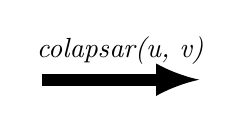
\begin{tikzpicture}
            \draw[-latex, thick, line width=1.5mm, above] (0,.5) -- node {\textit{colapsar(u, v)}} (2,.5);
        \end{tikzpicture}
        \begin{tikzpicture}[state/.style={circle}]
            % \tikzstyle{every state}=[circle,thick,minimum size=5mm, text=black,minimum width=1cm]
            \node[state] (u) {$u$};
            \node[circle,fill,inner sep=1.5pt] (su) [below left = 1.25cm and 0.5cm of u] {};
            \node[circle,fill,inner sep=1.5pt] (sv) [below right = 1.25cm and 0.5cm of u] {};
            \node[state] (p1) [above left = 1.25cm and 0.5cm of u] {$p1$};
            \node[state] (p2) [above = 1cm of u] {$p2$};
            \node[state] (p3) [above right = 1.25cm and 0.5cm of u] {$p3$};
            
            \path[-latex]  (p1) edge [thick, left] node {0} (u);
            \path[-latex]  (u) edge [thick, left] node {1} (su);
            \path[-latex]  (p2) edge [thick, left] node {0} (u);
            \path[-latex]  (p3) edge [thick, right] node {0} (u);
            \path[-latex]  (u) edge [thick, right] node {2} (sv);
            \path[-latex]  (su) edge [thick, left, dashed, bend left=20] node {0;1} (p1);
            \path[-latex]  (sv) edge [thick, left, dashed, bend right=50] node {0;2} (p2);
            \path[-latex]  (sv) edge [thick, right, dashed, bend right=50] node {0;2} (p3);
        \end{tikzpicture}
    \end{center}
    
    \begin{center}
        \begin{tikzpicture}[state/.style={circle}]
            % \tikzstyle{every state}=[circle,thick,minimum size=5mm, text=black,minimum width=1cm]
            \node[circle,fill,inner sep=1.5pt] (su) {};
            \node[state] (u) [above = 1cm of su] {$u$};
            \node[state] (p1) [above left = 1.25cm and 0.2cm of u] {$p2$};
            \node[state] (p2) [above right = 1.25cm and 0.2cm of u] {$p3$};
            
            \node[circle,fill,inner sep=1.5pt] (sv) [right = 1.5cm of su] {};
            \node[state] (v) [above = 1cm of sv] {$v$};
            
            \path[-latex]  (p1) edge [thick, left] node {0} (u);
            \path[-latex]  (u) edge [thick, left] node {0} (su);
            \path[-latex]  (p2) edge [thick, right] node {0} (u);
            \path[-latex]  (v) edge [thick, left] node {0} (sv);
        \end{tikzpicture}
        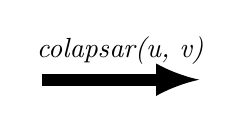
\begin{tikzpicture}
            \draw[-latex, thick, line width=1.5mm, above] (0,.5) -- node {\textit{colapsar(u, v)}} (2,.5);
        \end{tikzpicture}
        \begin{tikzpicture}[state/.style={circle}]
            % \tikzstyle{every state}=[circle,thick,minimum size=5mm, text=black,minimum width=1cm]
            \node[state] (u) {$u$};
            \node[circle, fill, inner sep=1.5pt] (su) [below left = 1.25cm and 0.5cm of u] {};
            \node[circle, fill, inner sep=1.5pt] (sv) [below right = 1.25cm and 0.5cm of u] {};
            \node[state] (p1) [above left = 1.25cm and 0.5cm of u] {$p1$};
            \node[state] (p2) [above right = 1.25cm and 0.5cm of u] {$p2$};
            
            \path[-latex]  (p1) edge [thick, left] node {0} (u);
            \path[-latex]  (u) edge [thick, left] node {1} (su);
            \path[-latex]  (p2) edge [thick, right] node {0} (u);
            \path[-latex]  (u) edge [thick, right] node {0} (sv);
            \path[-latex]  (su) edge [thick, left, dashed, bend left=20] node {0;1} (p1);
        \end{tikzpicture}
    \end{center}
    
    Cada aresta de ancestralidade possui como rótulo a informação necessária para refazer o caminho entre o destino e a origem através das arestas de dedução, esse caminho é identificado através das cores das arestas de dedução. Se o vértice possui premissas antes do colapso, é necessário atribuir uma cor para sua respectiva aresta dedutiva de saída após o colapso. Todas as arestas de dedução que saem de um determinado vértice possuem cores distintas, exceto para a cor 0.
    
    \item \textbf{Arestas de ancestralidade incidentes} \\
    Caso algum dos vértices a serem colapsados possua uma aresta de ancestralidade incidente, é necessário atualizar o destino e consequentemente o rótulo da aresta. Se o vértice possuir premissas, a aresta de ancestralidade é redirecionada para as premissas, caso contrário, a aresta é redirecionada para o vértice imediatamente inferior.
    
    \begin{center}
        \begin{tikzpicture}[state/.style={circle}]
            % \tikzstyle{every state}=[circle,thick,minimum size=5mm, text=black,minimum width=1cm]
            \node[state] (u) {$u$};
            \node[state] (v) [right = 0.5cm of u] {$v$};
            
            \node[state] (p1) [above left = 1.25cm and 0.2cm of u] {$p1$};
            \node[state] (p2) [above right = 1.25cm and 0.2cm of u] {$p2$};
            \node[circle,fill,inner sep=1.5pt] (su) [below = 1cm of u] {};
            \node[circle,fill,inner sep=1.5pt] (ssu) [below = 1cm of su] {};
            
            \node[circle,fill,inner sep=1.5pt] (sv) [below = 1cm of v] {};
            \node[circle,fill,inner sep=1.5pt] (ssv) [below = 1cm of sv] {};
            
            \path[-latex]  (p1) edge [thick, left] node {0} (u);
            \path[-latex]  (p2) edge [thick, right] node {0} (u);
            \path[-latex]  (u) edge [thick, right] node {0} (su);
            \path[-latex]  (su) edge [thick, dotted, right] node {s1} (ssu);
            \path[-latex]  (ssu) edge [thick, dashed, left, bend left = 30] node {0;s1} (u);
            
            \path[-latex]  (v) edge [thick, left] node {0} (sv);
            \path[-latex]  (sv) edge [thick, dotted, left] node {s2} (ssv);
            \path[-latex]  (ssv) edge [thick, dashed, right, bend right = 30] node {0;s2} (v);
        \end{tikzpicture}
        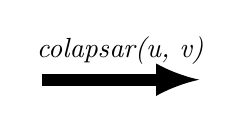
\begin{tikzpicture}
            \draw[-latex, thick, line width=1.5mm, above] (0,.5) -- node {\textit{colapsar(u, v)}} (2,.5);
        \end{tikzpicture}
        \begin{tikzpicture}[state/.style={circle}]
            % \tikzstyle{every state}=[circle,thick,minimum size=5mm, text=black,minimum width=1cm]
            \node[state] (u) {$u$};
            
            \node[state] (p1) [above left = 1.25cm and 0.2cm of u] {$p1$};
            \node[state] (p2) [above right = 1.25cm and 0.2cm of u] {$p2$};
            \node[circle,fill,inner sep=1.5pt] (su) [below left = 1.25cm and 0.3cm of u] {};
            \node[circle,fill,inner sep=1.5pt] (ssu) [below = 1cm of su] {};
            
            \node[circle,fill,inner sep=1.5pt] (sv) [below right = 1.25cm and 0.3cm of u] {};
            \node[circle,fill,inner sep=1.5pt] (ssv) [below = 1cm of sv] {};
            
            \path[-latex]  (p1) edge [thick, left] node {0} (u);
            \path[-latex]  (p2) edge [thick, right] node {0} (u);
            \path[-latex]  (u) edge [thick, left] node {1} (su);
            \path[-latex]  (su) edge [thick, dotted, right] node {s1} (ssu);
            \path[-latex]  (ssu) edge [thick, dashed, left, bend left = 60] node {0;1;s1} (p1);
            \path[-latex]  (ssu) edge [thick, dashed, left, bend left = 30] node {0;1;s1} (p2);
            
            \path[-latex]  (u) edge [thick, right] node {0} (sv);
            \path[-latex]  (sv) edge [thick, dotted, left] node {s2} (ssv);
            \path[-latex]  (ssv) edge [thick, dashed, right, bend right = 50] node {s2} (sv);
        \end{tikzpicture}
    \end{center}
    
    \item \textbf{Colapso de arestas} \\
    Nem sempre os destinos das arestas de dedução que saem dos vértices a serem colapsados possuem destinos diferentes. Caso os destinos já tenham sido colapsados no nível inferior, além de colapsar os vértices, é necessário colapsar as arestas.
    
    \begin{center}
        \begin{tikzpicture}[state/.style={circle}]
            % \tikzstyle{every state}=[circle,thick,minimum size=5mm, text=black,minimum width=1cm]
            \node[state] (u) {$u$};
            \node[state] (v) [right = 1cm of u] {$v$};
            
            \node[state] (p1) [above left = 1.25cm and 0.2cm of u] {$p1$};
            \node[state] (p2) [above right = 1.25cm and 0.2cm of u] {$p2$};
            \node[circle,fill,inner sep=1.5pt] (s) [below right = 1.25cm and 0.2cm of u] {};
            \node[circle,fill,inner sep=1.5pt] (ssu) [below = 1cm of s] {};
            
            \path[-latex]  (p1) edge [thick, left] node {0} (u);
            \path[-latex]  (p2) edge [thick, right] node {0} (u);
            \path[-latex]  (u) edge [thick, left] node {1} (s);
            \path[-latex]  (s) edge [thick, dotted, right] node {s1} (ssu);
            \path[-latex]  (ssu) edge [thick, dashed, left, bend left = 70] node {0;1;s1} (p1);
            \path[-latex]  (ssu) edge [thick, dashed, left, bend left = 45] node {0;1;s1} (p2);
            
            \path[-latex]  (v) edge [thick, right] node {0} (s);
        \end{tikzpicture}
        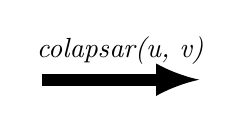
\begin{tikzpicture}
            \draw[-latex, thick, line width=1.5mm, above] (0,.5) -- node {\textit{colapsar(u, v)}} (2,.5);
        \end{tikzpicture}
        \begin{tikzpicture}[state/.style={circle}]
            % \tikzstyle{every state}=[circle,thick,minimum size=5mm, text=black,minimum width=1cm]
            \node[state] (u) {$u$};
            
            \node[state] (p1) [above left = 1.25cm and 0.2cm of u] {$p1$};
            \node[state] (p2) [above right = 1.25cm and 0.2cm of u] {$p2$};
            \node[circle,fill,inner sep=1.5pt] (s) [below = 1cm of u] {};
            \node[circle,fill,inner sep=1.5pt] (ssu) [below = 1cm of s] {};
            
            \path[-latex]  (p1) edge [thick, left] node {0} (u);
            \path[-latex]  (p2) edge [thick, right] node {0} (u);
            \path[-latex]  (u) edge [thick, right] node {$\lambda_{\{0,1\}}$} (s);
            \path[-latex]  (s) edge [thick, dotted, right] node {s1} (ssu);
            \path[-latex]  (ssu) edge [thick, dashed, left, bend left = 70] node {0;1;s1} (p1);
            \path[-latex]  (ssu) edge [thick, dashed, left, bend left = 45] node {0;1;s1} (p2);
        \end{tikzpicture}
    \end{center}
    
    $\lambda$ é a cor especial utilizada para indicar que a aresta foi colapsada. As arestas colapsadas ainda mantêm a informação das cores originais das arestas.
    
\end{itemize}

% \section{Dedução Natural Contextual}

% Proposta por Paleo em \cite{NDcPaleo}, a Dedução Natural Contextual (DNc) é um cálculo de dedução natural para M$\supset$ que utiliza \textit{deep inference}, o que permite aplicar as regras de dedução diretamente nas subfórmulas. Para alguns teoremas, a DNc é capaz de gerar provas quadraticamente menores que a dedução natural usual. Levando em consideração o isomorfismo de Curry-Howard entre a dedução natural da lógica intuicionista e o $\lambda$-$calculus$ simplesmente tipado, NDc é definido através do $\lambda_{c}$-$calculus$, uma extensão do $\lambda$-$calculus$ simplesmente tipado.

% Proposto por Alonzo Church em 1940, o $\lambda$-$calculus$ é um sistema formal voltado para a representação de funções computáveis.

% \begin{definition}{\textbf{$\lambda$-termos.}}
% Seja um conjunto infinito de variáveis $\{x, y, ...\}$, o conjunto de $\lambda$-termos é definido como segue:

% \begin{enumerate}
%     \item Toda variável é um $\lambda$-termo.
%     \item Se $x$ é uma variável e A é um $\lambda$-termo, $\lambda{x}.A$ é um $\lambda$-termo.
%     \item Se A e B são $\lambda$-termos, $(A B)$ é um $\lambda$-termo.
% \end{enumerate}
% \end{definition}

% Em sua versão tipada, cada termo do $\lambda$-$calculus$ possui um tipo associado. Seja o conjunto de variáveis de tipos $\{\alpha, \beta, ...\}$, as \textit{declarações de tipos} $$t:\alpha$$ $$t^{\alpha}$$ declaram que o termo $t$ possui o tipo $\alpha$, e $$t: \alpha \rightarrow \beta$$ declara que $t$ é uma função que transforma um argumento do tipo $\alpha$ em um argumento do tipo $\beta$. Os tipos de cada termo são definidos através das \textit{regras de tipagem} utilizando as \textit{relações de tipagem}. A relação de tipagem $$\Gamma \vdash t: \alpha$$ informa que no contexto de tipagem $\Gamma$ o termo $t$ possui tipo $\alpha$, o contexto de tipagem $\Gamma$ é um conjunto de declarações de tipos. Seja $\mathcal{I}$ um isomorfismo entre o $\lambda$-$calculus$ simplesmente tipado e a dedução natural de M$\supset$, onde um $\lambda$-termo com tipo $\alpha$ corresponde a prova do teorema $\alpha$ em M$\supset$, as regras de inferência da dedução natural de M$\supset$ correspondem as regras de tipagem do $\lambda$-$calculus$ simplesmente tipado (Figura \ref{fig:tip_lambda}).

% \begin{figure}[ht]
%     \begin{center}
%         \begin{minipage}[t][25mm][t]{130mm}
%             \begin{prooftree}
%                 \AxiomC{}
%                 \UnaryInfC{$\Gamma, a: \alpha \vdash a: \alpha$}
%             \end{prooftree}
%         \end{minipage}
%         \begin{minipage}[t][25mm][t]{65mm}
%             \begin{prooftree}
%                 \AxiomC{$\Gamma, a: \alpha \vdash b: \beta$}
%                 \RightLabel{$\mysupset{-I}$}
%                 \UnaryInfC{$\Gamma \vdash \lambda{a^{\alpha}}.b: \alpha \rightarrow \beta$}
%             \end{prooftree}
%         \end{minipage}
%         \hfill
%         \begin{minipage}[t][25mm][t]{65mm}
%             \begin{prooftree}
%                 \AxiomC{$\Gamma \vdash f: \alpha \rightarrow \beta$}
%                 \AxiomC{$\Gamma \vdash a: \alpha$}
%                 \RightLabel{$\mysupset{-E}$}
%                 \BinaryInfC{$\Gamma \vdash (f a): \beta$}
%             \end{prooftree}
%         \end{minipage}
%     \caption{Regras de tipagem (inferência) do $\lambda$-$calculus$ simplesmente tipado (da dedução natural para M$\supset$)}
%     \label{fig:tip_lambda}
%     \end{center}
% \end{figure}

% A DNc aplica as regras de inferência diretamente nas subfórmulas. Seja $\alpha$ uma fórmula, $\mathcal{C}_{\pi}[\alpha]$ representa a subfórmula de $\alpha$ na posição $\pi$, $\mathcal{C}_{\pi}[\_]$ é o contexto de $\alpha$. Seja uma representação em árvore binária da fórmula $\alpha$, onde cada implicação é uma ramificação, a posição $\pi$ é representada por uma cadeia de \textit{bits} que representa o caminho da raiz de $\mathcal{C}_{\pi}[\alpha]$ até $\alpha$. As regras de inferência da DNc são mostradas na Figura \ref{fig:tip_DNc}.

% \begin{figure}[ht]
%     \begin{center}
%         \begin{minipage}[t][25mm][t]{130mm}
%             \begin{prooftree}
%                 \AxiomC{}
%                 \UnaryInfC{$\Gamma, a: \alpha \vdash a: \alpha$}
%             \end{prooftree}
%         \end{minipage}
%         \begin{minipage}[t][25mm][t]{130mm}
%             \begin{prooftree}
%                 \AxiomC{$\Gamma, a: \alpha \vdash b: \mathcal{C_{\pi}}[\beta$]}
%                 \RightLabel{$\mysupset{-I}$}
%                 \UnaryInfC{$\Gamma \vdash \lambda{a^{\alpha}}.b: \mathcal{C_{\pi}}[\alpha \rightarrow \beta]$}
%             \end{prooftree}
%         \end{minipage}
%         \hfill
%         \begin{minipage}[t][25mm][t]{130mm}
%             \begin{prooftree}
%                 \AxiomC{$\Gamma \vdash f: \mathcal{C}_{\pi1}^1[\alpha \rightarrow \beta]$}
%                 \AxiomC{$\Gamma \vdash a: \mathcal{C}_{\pi2}^2[\alpha]$}
%                 \RightLabel{$\mysupset{-E^\rightharpoonup}$}
%                 \BinaryInfC{$\Gamma \vdash (f$ $a)_{(\pi1;\pi2)}^{\rightharpoonup}: \mathcal{C}_{\pi1}^1[\mathcal{C}_{\pi2}^2[\beta]]$}
%             \end{prooftree}
%         \end{minipage}
%         \begin{minipage}[t][25mm][t]{130mm}
%             \begin{prooftree}
%                 \AxiomC{$\Gamma \vdash f: \mathcal{C}_{\pi1}^1[\alpha \rightarrow \beta]$}
%                 \AxiomC{$\Gamma \vdash a: \mathcal{C}_{\pi2}^2[\alpha]$}
%                 \RightLabel{$\mysupset{-E^\leftharpoonup}$}
%                 \BinaryInfC{$\Gamma \vdash (f$ $a)_{(\pi1;\pi2)}^{\leftharpoonup}: \mathcal{C}_{\pi2}^2[\mathcal{C}_{\pi1}^1[\beta]]$}
%             \end{prooftree}
%         \end{minipage}
%     \caption{Regras de tipagem (inferência) do $\lambda_{c}$-$calculus$ (da DNc)}
%     \label{fig:tip_DNc}
%     \end{center}
% \end{figure}

% Existem duas regras de eliminação da implicação, uma para cada possibilidade de combinação dos contextos. Essa peculiaridade pode tornar a implementação de provadores de teoremas para NDc mais complexas e, consequentemente, mais lentas.

% A completude e a corretude são mostradas através de traduções em ambos os sentidos de provas de teoremas em dedução natural usal e NDc, os detalhes dessas traduções não fazem parte do escopo deste trabalho.

% \section{Compressão de Dados}

\section{Codificação de Huffman}

Proposta em 1952 por David Huffman \cite{huffman1952}, a \textit{Codificação de Huffman} é uma técnica de compressão de dados sem perdas, que permite recuperar o dado original a partir do dado comprimido, baseada na substituição de símbolos do dado por códigos. O objetivo é minimizar a quantidade de espaço necessário para representar o dado atribuindo códigos menores para os símbolos mais frequentes e códigos maiores para os menos frequentes. Para otimizar o uso do espaço, normalmente, utiliza-se uma codificação binária para comprimir os dados, no entanto, a codificação de Huffman é extensível para codificações n-árias. 

\theoremstyle{definition}
\begin{definition}{\textbf{Codificação binária.}}
Seja uma mensagem \textit{m} com um alfabeto $\Sigma$, uma \textit{codificação binária} é uma função $F$ que mapeia cada símbolo de $\Sigma$ em uma cadeia de bits, $F: \Sigma \rightarrow \{0, 1\}^*$, tal que:

\begin{enumerate}
    \item Para todo símbolo $a \in \Sigma$, $F(a) \neq \epsilon$, $F(a)$ não é vazia.
    \item Para todos símbolos $a, b \in \Sigma$, $F(a) \neq F(b)$.
    \item Para todos símbolos $a, b \in \Sigma$, $F(a)$ não é prefixo de $F(b)$.
\end{enumerate}
\end{definition}

A condição (3) permite que, dada uma mensagem $m = \langle a_1, ..., a_n \rangle$ e uma codificação binária $F$, a mensagem codificada $m_c = \langle F(a_1), ..., F(a_n) \rangle$ seja decodificada sem informações adicionais. Por exemplo, seja uma mensagem $babcb$ e uma codificação binária, $F(a) = 111$, $F(b) = 010$ e $F(c) = 000$. Uma mensagem codificada $010111010000010$ possui apenas uma segmentação possível baseada na codificação binária do alfabeto, $010|111|010|000|010$, que corresponde exatamente a mensagem original $babcb$.

A construção da codificação binária utilizada por Huffman é baseada na probabilidade de ocorrência dos símbolos do alfabeto na mensagem a ser codificada, utilizando tabelas auxiliares para atribuir códigos a cada símbolo do alfabeto. Seja $(s, p)$, um símbolo e sua respectiva probabilidade de ocorrência, a construção das tabelas auxiliares segue os seguintes passos:

\begin{enumerate}
    \item Inicialmente, uma tabela com todos os símbolos e suas respectivas probabilidades é criada, as entradas são ordenadas em ordem decrescente das probabilidades.
    \item Seleciona as entradas com as menores probabilidades, $(s_1, p_1)$ e $(s_2, p_2)$, cria uma entrada auxiliar $((s_1, s_2), p_1+p_2)$ e adiciona em uma nova tabela com as entradas de todos os símbolos, exceto $s_1$ e $s_2$.
    \item Repete o passo 2 até que a tabela criada tenha apenas uma entrada.
\end{enumerate}

A Figura \ref{fig:exe_tab_aux} mostra um exemplo de criação das tabelas auxiliares do alfabeto $\Sigma = \{a, r, j, l, m, p\}$, onde as probabilidades de $a, r, j, l, m$ e $p$ são, respectivamente, 0.35, 0.20, 0.15, 0.13, 0.12 e 0.05. Para facilitar a visualização, as entradas auxiliares estão destacadas em negrito.

\begin{figure}[ht]
    \begin{center}
        \begin{tikzpicture}
        [every node/.style={minimum height=2em}]
        \matrix [matrix of math nodes](Mat)
        {
        |[minimum width=1.8em]|& T1 &|[minimum width=1.8em]| & T2 &|[minimum width=1.8em]|& T3 &|[minimum width=1.8em]|& T4 &|[minimum width=1.8em]|& T5 &|[minimum width=1.8em]|& T6\\
        & 0.35 && 0.35           && 0.35          && \textbf{0.37} && \textbf{0.63} && \textbf{1.00}\\
        & 0.20 && 0.20           && \textbf{0.28} && 0.35          && \textbf{0.37} &&     \\
        & 0.15 && \textbf{0.17}  && 0.20          && \textbf{0.28} &&               &&     \\
        & 0.13 && 0.15           && \textbf{0.17} &&               &&               &&     \\
        & 0.12 && 0.13           &&               &&               &&               &&     \\
        & 0.05 && &              &&               &&               &&               &&     \\
        };
        
        \draw[-latex] (Mat-7-2.east) -- (Mat-4-4);
        \draw[-latex] (Mat-6-2.east) -- (Mat-4-4);
        \draw[-latex] (Mat-5-4.east) -- (Mat-3-6);
        \draw[-latex] (Mat-6-4.east) -- (Mat-3-6);
        \draw[-latex] (Mat-4-6.east) -- (Mat-2-8);
        \draw[-latex] (Mat-5-6.east) -- (Mat-2-8);
        \draw[-latex] (Mat-3-8.east) -- (Mat-2-10);
        \draw[-latex] (Mat-4-8.east) -- (Mat-2-10);
        \draw[-latex] (Mat-2-10.east) -- (Mat-2-12);
        \draw[-latex] (Mat-3-10.east) -- (Mat-2-12);
        \end{tikzpicture}
        \caption{Exemplo de tabelas auxiliares da codificação de Huffman}
        \label{fig:exe_tab_aux}
    \end{center}
\end{figure}

A partir das tabelas auxiliares é possível construir uma árvore binária para a obtenção do código de cada símbolo, tal construção ocorre percorrendo as tabelas na direção inversa da criação, onde a raiz da árvore é a entrada auxiliar com probabilidade igual a 1.0 da última tabela e as folhas são as entradas originais (tabela T1) das probabilidades dos símbolos do alfabeto. Para cada fusão de entradas realizada pelo passo 2 é criada uma ramificação na árvore, onde a entrada com a menor probabilidade é atribuída ao filho direito e a entrada com maior probabilidade é atribuída ao filho esquerdo. Cada arco da árvore é rotulado com 1 ou 0, os arcos dos filhos esquerdos e direitos são rotulados, respectivamente, com 0 e 1. A Figura \ref{fig:exe_arv_bin} mostra a árvore criada a partir das tabelas da Figura \ref{fig:exe_tab_aux}.

\begin{figure}[!ht]
    \begin{center}
        \begin{tikzpicture}[auto, elliptic state/.style={draw,ellipse}]
            % \tikzstyle{every state}=[circle,thick,minimum size=5mm, text=black,minimum width=1cm]
            \node[elliptic state] (root) {1.0};
            \node[elliptic state] [below left = 1.5cm and 2.5cm of root] (l) {0.63};
            \node[elliptic state, fill = backcolour2] (ll) [below left = 1.5cm and 0.7cm of l] {0.35 [a]};
            \node[elliptic state] (lr) [below right = 1.5cm and 0.7cm of l] {0.28};
            \node[elliptic state, fill = backcolour2] (lrl) [below left = 1.5cm and 0.1cm of lr] {0.15 [j]};
            \node[elliptic state, fill = backcolour2] (lrr) [below right = 1.5cm and 0.1cm of lr] {0.13 [l]};
            \node[elliptic state] (r) [below right = 1.5cm and 2.5cm of root] {0.37};
            \node[elliptic state, fill = backcolour2] (rl) [below left = 1.5cm and 0.7cm of r] {0.20 [r]};
            \node[elliptic state] (rr) [below right = 1.5cm and 0.7cm of r] {0.17};
            \node[elliptic state, fill = backcolour2] (rrl) [below left = 1.5cm and 0.1cm of rr] {0.12 [m]};
            \node[elliptic state, fill = backcolour2] (rrr) [below right = 1.5cm and 0.1cm of rr] {0.05 [p]};
            
            % \node[state, inner sep=1mm,minimum size=1.2cm, label=right:$w_2$] (C) [above right of=A] {$\alpha \supset \beta$};
            
            \path[-latex]  (root) edge [thick, above left] node {0} (l);
            \path[-latex]  (root) edge [thick] node {1} (r);
            \path[-latex]  (l) edge [thick] node {1} (lr);
            \path[-latex]  (l) edge [thick, above left] node {0} (ll);
            \path[-latex]  (lr) edge [thick, above left] node {0} (lrl);
            \path[-latex]  (lr) edge [thick] node {1} (lrr);
            \path[-latex]  (r) edge [thick] node {1} (rr);
            \path[-latex]  (r) edge [thick, above left] node {0} (rl);
            \path[-latex]  (rr) edge [thick, above left] node {0} (rrl);
            \path[-latex]  (rr) edge [thick] node {1} (rrr);
        \end{tikzpicture}
        \caption{Exemplo de árvore binária criada a partir das tabelas auxiliares da codificação de Huffman}
        \label{fig:exe_arv_bin}
    \end{center}
\end{figure}

Os códigos de cada símbolo são obtidos percorrendo os caminhos da raiz até cada folha e armazenando os rótulos dos arcos percorridos. A Tabela \ref{tab:cod_huf} mostra os códigos obtidos da árvore da Figura \ref{fig:exe_arv_bin}. Os símbolos com as maiores probabilidades, 'a' e 'r', ficaram com os menores códigos, respectivamente, 00 e 10. 

\begin{table} [!ht]
    \caption{Exemplos de códigos obtidos a partir da árvore binária da codificação de Huffman.}\label{tab:cod_huf}
    ~\\[-2mm]
    \begin{tabularx}{\textwidth}{@{\extracolsep{0pt}}C @{\extracolsep{0pt}}C C C}

        \textbf{Símbolo}
        & \textbf{Probabilidade}
        & \textbf{Código}
        \\\toprule

        ~ \\[-6mm]
        a
        & 0.35
        & 00
        \\\midrule
    
        ~ \\[-6mm]
        r
        & 0.20
        & 10
        \\\midrule
    
         ~ \\[-6mm]
        j
        & 0.15
        & 010
        \\\midrule
    
         ~ \\[-6mm]
        l
        & 0.13
        & 011
        \\\midrule
        
         ~ \\[-6mm]
        m
        & 0.12
        & 110
        \\\midrule
        
         ~ \\[-6mm]
        p
        & 0.05
        & 111
        \\\midrule
    \end{tabularx}
\end{table}